\chapter{Methodology}%
\label{chapter:methodology}

\begin{introduction}
This chapter presents the non-functional requirements and the use cases of the applications. 
\end{introduction} 




\section{Application Requirements}
The requirements for the application were identified using the FURPS model, which divides requirements into functional and non-functional categories.

\subsection{Non-Functional Requirements}
The main non-functional requirements, organized by FURPS, are summarized as follows:

\begin{table}[htbp]
\centering
\begin{tabular}{|l|p{10cm}|}
\hline
\textbf{Category} & \textbf{Requirement} \\ \hline
Scalability & The system should be able to support users from Europe. \\ \hline
Reliability & The system should have an availability of 99\% and must recover from any failure within 4 hours. \\ \hline
Performance & The system should not take longer than 2 seconds to respond. \\ \hline
Usability & Training for a new user should not take longer than 8 hours. \\ \hline
Supportability & The system should be compatible with Chrome, Firefox, Microsoft Edge, and Safari browsers. \\ \hline
\end{tabular}
\caption{Non-Functional Requirements (FURPS Model)}
\end{table}

\subsection{Functional Requirements}
The application supports the following user roles: receptionist, mechanic, warehouse manager, and workshop manager. There is also a client application and an administrator view.

\subsubsection{Administrator}
\begin{itemize}
    \item Create, edit, view, and remove task types
    \item Manage dealerships (create, edit, view, remove, add/remove vehicle types)
    \item Manage vehicle parts (create, edit, view, remove)
    \item Create and view dealership employees
\end{itemize}

\subsubsection{Receptionist}
\begin{itemize}
    \item Switch interface language between English and Portuguese
    \item View daily working hours and user-specific hours
    \item Schedule vehicle reception (registration number, client email, owner name, reception date)
    \item Create maintenance (expected budget, tasks, expected conclusion date)
    \item View active maintenances (client name, registration number, entity, creation date, evaluation date, expected conclusion date, budget, planned work hours, tasks)
    \item Receive notifications on budget or deadline changes in maintenance
    \item Confirm or reject maintenance changes
    \item Cancel maintenance
    \item Conclude maintenance
    \item Notify when all maintenance tasks are completed
\end{itemize}

\subsubsection{Mechanic}
\begin{itemize}
    \item Switch interface language between English and Portuguese
    \item View today’s tasks
    \item Pause and continue tasks (e.g., for breaks)
    \item View maintenance task details (registration number, task type, parts, step descriptions, needed parts, client desired tasks)
    \item Finalize a task and comment before completion
    \item View evaluation tasks (maintenance tasks needed, client comment)
    \item If evaluations are not used, maintenance concludes when a mechanic finishes the evaluation task
\end{itemize}

\subsubsection{Warehouse Manager}
\begin{itemize}
    \item Switch interface language between English and Portuguese
    \item View dealership inventory (name, code, quantity, warehouse location, description, category, price, quantity per group, min/max values for alarms/purchase requests)
    \item Edit part type details (location, min/max values, purchase request quantities)
    \item View quantity changes over time for each part
    \item See supplier details (name, phone, email, address, contract parts with start/end date)
    \item Create purchase requests (motive, parts, quantity per part)
    \item View all purchases (status, arrival date, total price, motive, creation date, parts, stock quantity, price, associated tasks)
    \item Register expected arrival date or delays for purchases
    \item Finalize delivery purchase by registering received parts
\end{itemize}

\subsubsection{Workshop Manager}
\begin{itemize}
    \item Switch interface language between English and Portuguese
    \item View daily and user-specific working hours
    \item View unassigned tasks
    \item Assign tasks to mechanics
    \item View and manage active maintenances (full details including done/planned tasks)
    \item Add tasks to active maintenances
    \item View completed tasks with filters (client, vehicle, date), details (client name, vehicle registration, entity, creation date, evaluation date, conclusion date, budget, hours, price), and export as PDF
    \item View monthly maintenance revenue and total hours worked
    \item Assign purchases to operators
    \item View purchase requests (price, motive, creation date, parts info)
    \item Authorize or reject purchase requests
    \item Create supplier records (name, phone, email, address, contract parts/details)
    \item View suppliers and partnerships with bike sharing entities; accept/reject partnerships
    \item View employee list (email, name, DOB, phone, sex, role); create employee records (all listed data plus password)
\end{itemize}


\subsubsection{Client}
\begin{itemize}
    \item View active maintenance information
    \item View maintenance history
    \item evaluate the perception of the service quality 
    \item evaluate the expected service quality 
\end{itemize}


\subsection{System Requirements}
The system also enforces several logical and structural requirements, detailed as follows:
\begin{itemize}
    \item The system must generate a repair report for each maintenance completed.
    \item Each maintenance task must have a defined sequence to ensure correct order of execution.
    \item Each purchase record may include multiple parts, along with their respective details.
\end{itemize}

A dealership can only create maintenance of vehicle from bike sharing entities that are there partners, otherwise it can only accept maintenance from clients with no entity.
The system should be flexible and handle general flow of a vehicle maintenance and the workflow of \ac{emel}.  

\section{Applications use Cases} 
I developed a set of use cases for each user.

The receptionist will be responsible for interacting with the client, this includes the vehicle check-in and check-out and user communication. 
The use cases are:

\begin{itemize}
    \item Use Case 1.1 – Maintenance Schedule
    \begin{itemize}
      \item Scenario – The client arrives at the dealership with a vehicle to be repaired.
      \item Objective – Create a new maintenance request in the system.
      \item System – The receptionist fills a form with the vehicle registration, the evaluation date, the entity associated, the client email, client notes and tasks requested by the user
    \end{itemize}
        \item Use Case 1.2 – Define maintenance details
    \begin{itemize}
      \item Scenario – The vehicle evaluation has terminated
      \item Objective – Define the budget, a conclusion date and the tasks to be performed.
      \item System – The receptionist receives a notification that the vehicle evaluation is complete and, together with the customer, determines which tasks have to be performed. The system calculates the price, and the receptionist sets a completion date.
    \end{itemize}
    \item Use Case 1.3 – Collect information about a maintenance request
    \begin{itemize}
      \item Scenario – A Client calls the dealership to ask about the maintenance of his vehicle.
      \item Objective – Visualize the maintenance information.
      \item System –  The Receptionist searches a list of maintenance requests by vehicle or customer and he can visualize the details of the selected maintenance.
    \end{itemize}
    \item Use Case 1.4 – Accept maintenance changes
    \begin{itemize}
      \item Scenario – A problem in a vehicle maintenance has occurred and the initial agreement with the client was broken, but the client accepts the changes.
      \item Objective – Accept the changes of the maintenance.
      \item System – The Receptionist goes to the maintenance details, to the section of the maintenance changes and accept the changes for that maintenance.
    \end{itemize}
    \item Use Case 1.5 – Refuse maintenance changes
    \begin{itemize}
      \item Scenario – A problem in a vehicle maintenance has occurred and the initial agreement with the client was broken and the client refuses the changes.
      \item Objective – Refuse the changes of the maintenance.
      \item System – The Receptionist goes to the maintenance details, to the section of the maintenance changes and refuses the changes for that maintenance.
    \end{itemize}
      \item Use Case 1.6 – Vehicle Delivery 
    \begin{itemize}
      \item Scenario – The Receptionist delivered the vehicle to the Client.
      \item Objective – Complete the vehicle maintenance process.
      \item System – Sends a report in a PDF format to the client with the information about the maintenance and alters the maintenance request status in the system to conclude. 
    \end{itemize}
      \item Use Case 1.7 – Cancel Maintenance 
    \begin{itemize}
      \item Scenario – The client does not like the maintenance agreement and wants to retreive the vehicle.
      \item Objective – Cancel the maintenance.
      \item System – The rececionist goes to the maintenance details and cancels the maintenance. 
    \end{itemize}
    \item Use Case 1.8 – Cancel Task 
    \begin{itemize}
      \item Scenario – A problem in a vehicle maintenance has occurred and the initial agreement with the client was broken and the client refuses the changes.
      \item Objective – Cancel the task to be done.
      \item System – The Receptionist goes to the maintenance details, to the section of the maintenance changes and cancels the task with the problem.
    \end{itemize}
  \end{itemize}  
  \hfill \break


 The mechanic will be responsible for doing the maintenance in the vehicle, like oil change, tire change, trade vehicle parts, etc. 
 The mechanic use cases are:

  \begin{itemize}
    \item Use Case 2.1 – View to-do list
    \begin{itemize}
      \item Scenario – The mechanic inicialize its shift.
      \item Objective – See tasks to be completed.
      \item System – The mechanic enters the system and encounters a list of tasks assigned to him and to be assign. Each task is accompanied by a description, a priority, a vehicle identification, a set of actions to be performed, and comments from other users. 
    \end{itemize}
    \item Use Case 2.2 – Carry out a vehicle analysis 
    \begin{itemize}
      \item Scenario – A new vehicle needs to be analyzed.
      \item Objective – Confirm the initial analysis of the receptionist and search for additional problems.
      \item System – The mechanic enters a list of tasks that need to be performed in the vehicle. 
    \end{itemize}
    \item Use Case 2.3 – Register tasks completed
    \begin{itemize}
      \item Scenario – A new vehicle needs maintenance.
      \item Objective – Complete maintenance
      \item System – The mechanic selects a list of tasks that he done on the vehicle.
    \end{itemize}
  \item Use Case 2.4 – Do a Vehicle maintenance task
  \begin{itemize}
    \item Scenario – A new vehicle is ready for maintenance.
    \item Objective – The mechanic will do a vehicle maintenance task (oil change, tire change, vehicle wash…).
    \item System – The mechanic starts a task and see a sequence of steps to complete the task. In the final step the mechanic can leave a note.
  \end{itemize}
  \item Use Case 2.5 – Change Task
  \begin{itemize}
    \item Scenario – A created task has the wrong part associated.
    \item Objective – Change the task to the correct part.
    \item System – It is registered a new task change that need to be approved by the workshop manager. In case the inicial budget or the maintenance schedule is altered, the client also needs to be notified and give authorization to change the task.
  \end{itemize}
    \item Use Case 2.6 – Continue Task
  \begin{itemize}
    \item Scenario – The mechanic leave the aplication before finishing the task
    \item Objective – Continue a task previously started.
    \item System – The mechanic can see a tasked paused in the list of the tasks he has to do. By clicking the continue button, the mechanic can continue the task.
  \end{itemize}
\end{itemize}
\hfill \break

The warehouse operator is responsible for managing the dealer's stock and asking for supplies. 
In this case, the use cases are as follows:

\begin{itemize}
  \item Use Case 3.1 – View the different parts that the warehouse possess
  \begin{itemize}
    \item Scenario – The warehouse worker wants to view the quantity of certain parts that the warehouse possesses.
    \item Objective – Show quantitative warehouse information.
    \item System – List of all parts and their quantities that the warehouse possesses. 
  \end{itemize}
  \item Use Case 3.2 – Requesting purchasing service 
  \begin{itemize}
    \item Scenario – The warehouse worker discovers that he has an insufficient number of parts for maintenance or anticipates that this part will be missing soon.
    \item Objective – Request permission to purchase parts from the supplier.
    \item System – The Warehouse Worker will place a purchase order for parts. The system notifies the administrator via the platform and by email requesting authorization to make the purchase. 
  \end{itemize}
    \item Use Case 3.3 – Buy new parts
  \begin{itemize}
    \item Scenario – The warehouse worker contacts the supplier to request new parts.
    \item Objective – Register the information of the new purchase.
    \item System – The warehouse operator introduce to the system the date that the parts will arrive.
  \end{itemize}
  \item Use Case 3.4 – Registration of new parts in the System
  \begin{itemize}
    \item Scenario – The warehouse worker purchased several parts from a supplier.
    \item Objective – Register new parts in the system.
    \item System – The warehouse operator adds to the system the parts that arrived to the warehouse and the date that the purchase is completed.
  \end{itemize}
    \item Use Case 3.5 – Edit Inventory 
  \begin{itemize}
    \item Scenario – The warehouse worker wants to change the part type information.
    \item Objective – Change the part type information.
    \item System – The warehouse operator can change the part type description, location, name or code.
  \end{itemize}
  \item Use Case 3.6 – Create Purchase Delay
  \begin{itemize}
    \item Scenario – A purchase has been delayed.
    \item Objective – Create a purchase delay.
    \item System – The warehouse operator goes to the purchase delay and inserts the new expected arrival date.
  \end{itemize}
\end{itemize}
\hfill \break

The last user of the application is the Workshop Manager. This user is in charge of managing the platform and the dealership. So the main use cases encountered are:

\begin{itemize}
    \item Use Case 4.1 – Assign tasks to the employees
  \begin{itemize}
    \item Scenario – A new maintenance request has been requested.
    \item Objective – Assign and organize tasks to different employees.
    \item System – The Workshop Manager assigns the various tasks of vehicle maintenance to the workshop employees.
  \end{itemize}
  \item Use Case 4.2 – Authorize purchase
  \begin{itemize}
    \item Scenario –  The Workshop Manager received a purchase request.
    \item Objective – Authorize or reject a purchase authorization request.
    \item System – The Workshop Manager can reject or authorize the maintenance request. 
  \end{itemize}
  \item Use Case 4.3 – View history of maintenance performed
  \begin{itemize}
    \item Scenario – The Workshop Manager wants to gather information from recently performed maintenance.
    \item Objective – View information about a specific maintenance that occurred.
    \item System – The Workshop Manager views a list of all maintenance that occurred as well as its details (who carried it out, which parts were removed, the name of the customer, tests carried out, and their results…). 
  \end{itemize}
  \item Use Case 4.4 – Develop statistics
  \begin{itemize}
    \item Scenario – The Workshop Manager wants to gather statistics on the maintenance that was carried out in the last month.
    \item Objective – View information about maintenance over a given period of time.
    \item System – Presentation graphs of the number of parts replaced, number of purchases, total price spent on new parts, remuneration for maintenance, average customer rating, etc.
  \end{itemize}
  \item Use Case 4.5 – Assign roles to employees
  \begin{itemize}
    \item Scenario – A new employee has been hired.
    \item Objective –  Assign roles to new employees.
    \item System – The Workshop Manager assigns to the new employee a certain role and set of permissions.
  \end{itemize}
  %   \item Use Case 4.6 – Authorize task change
  % \begin{itemize}
  %   \item Scenario – The Workshop Manager is notified with a new task change.
  %   \item Objective – Reject or authroize the new task change.
  %   \item System – The Workshop Manager assigns to the new employee a certain role and set of permissions.
  % \end{itemize}
  \item Use Case 4.6 – Add new Task
  \begin{itemize}
    \item Scenario – A task is missing in an on going maintenance.
    \item Objective – Add a new task to the on going maintenance.
    \item System – In the maintenance details the Workshop Manager sees a list of task that he can add to the maintenance. By adding the task, it needs to be validated by the client first.
  \end{itemize}
  \item Use Case 4.7 – Create Employee
  \begin{itemize}
    \item Scenario – A new employee has been hired for the workshop.
    \item Objective – Adding a new employee to the system.
    \item System – The workshop manager fill a form with the name of the new employee, the email, its role, phone number and date of birth .
  \end{itemize}
    \item Use Case 4.8 – Accept/Reject partnership
  \begin{itemize}
    \item Scenario – A new entity wants to work with the dealership to do the maintenance of there's vehicles .
    \item Objective – Associate the entity to the dealerships.
    \item System – Change the status of the request of the partnership request to "accept" or "rejected" depending of the warehouse manager choice.
  \end{itemize}

\end{itemize}
\hfill \break

The client application will only be interacted with by a role of users, the client.
The use cases are listed below:

\begin{itemize}
  \item Use Case 5.1 – View current maintenance status
  \begin{itemize}
    \item Scenario – The Customer wants to find information regarding the vehicle maintenance procedure.
    \item Objective – Display current maintenance status.
    \item System – The system will illustrate all the maintenance steps that the vehicle has already undergone, as well as those that remain to be completed. 
  \end{itemize}
  \item Use Case 5.2 – Notify the customer of the end of maintenance 
  \begin{itemize}
    \item Scenario – Vehicle maintenance has been completed and the customer can now collect the vehicle.
    \item Objective – Notify the user of the end of maintenance.
    \item System – The system will show an SMS/native notification on the customer's cell phone informing that the vehicle is ready to be picked up. 
  \end{itemize}
  \item Use Case 5.3 – Rating of the service provided
  \begin{itemize}
    \item Scenario – The client receives the vehicle and the receptionist completes the maintenance process.
    \item Objective – Get feedback from the client.
    \item System – The system will show a form to the client asking about the service provided. 
  \end{itemize}
    \item Use Case 5.4 – Rating of the service expected
  \begin{itemize}
    \item Scenario – After defining the agreement to the maintenance of the vehicle.
    \item Objective – The Client rating the quality of the service he is expected to receive.
    \item System – The system will show a form to the client asking about the service he is expected to receive. 
  \end{itemize}
      \item Use Case 5.5 – View maintenance history
  \begin{itemize}
    \item Scenario – The client wants to see the price of the last maintenance.
    \item Objective – See the information about the last maintenance of the client.
    \item System – The client opens the app and sees a page call "Maintenance History" in the menu. When clicking on tha page it shows a list of all the maintenances of that account. The client click on the first one, because it is ordered by date and it opens the details of the that maintenance in a offcanvas 
  \end{itemize}
\end{itemize}
\hfill \break



\section{Applications Workflow}

After the development of the use cases, a flow chart was designed to understand the users' interaction with the system and each other. The chart is visible in figure \ref{fig:figure2}.

\begin{figure}[h]
  \caption{Use Case Flow Chart of the Client, Receptionist, Mechanic, Warehouse Operator, and Administrator.}
  \centering
  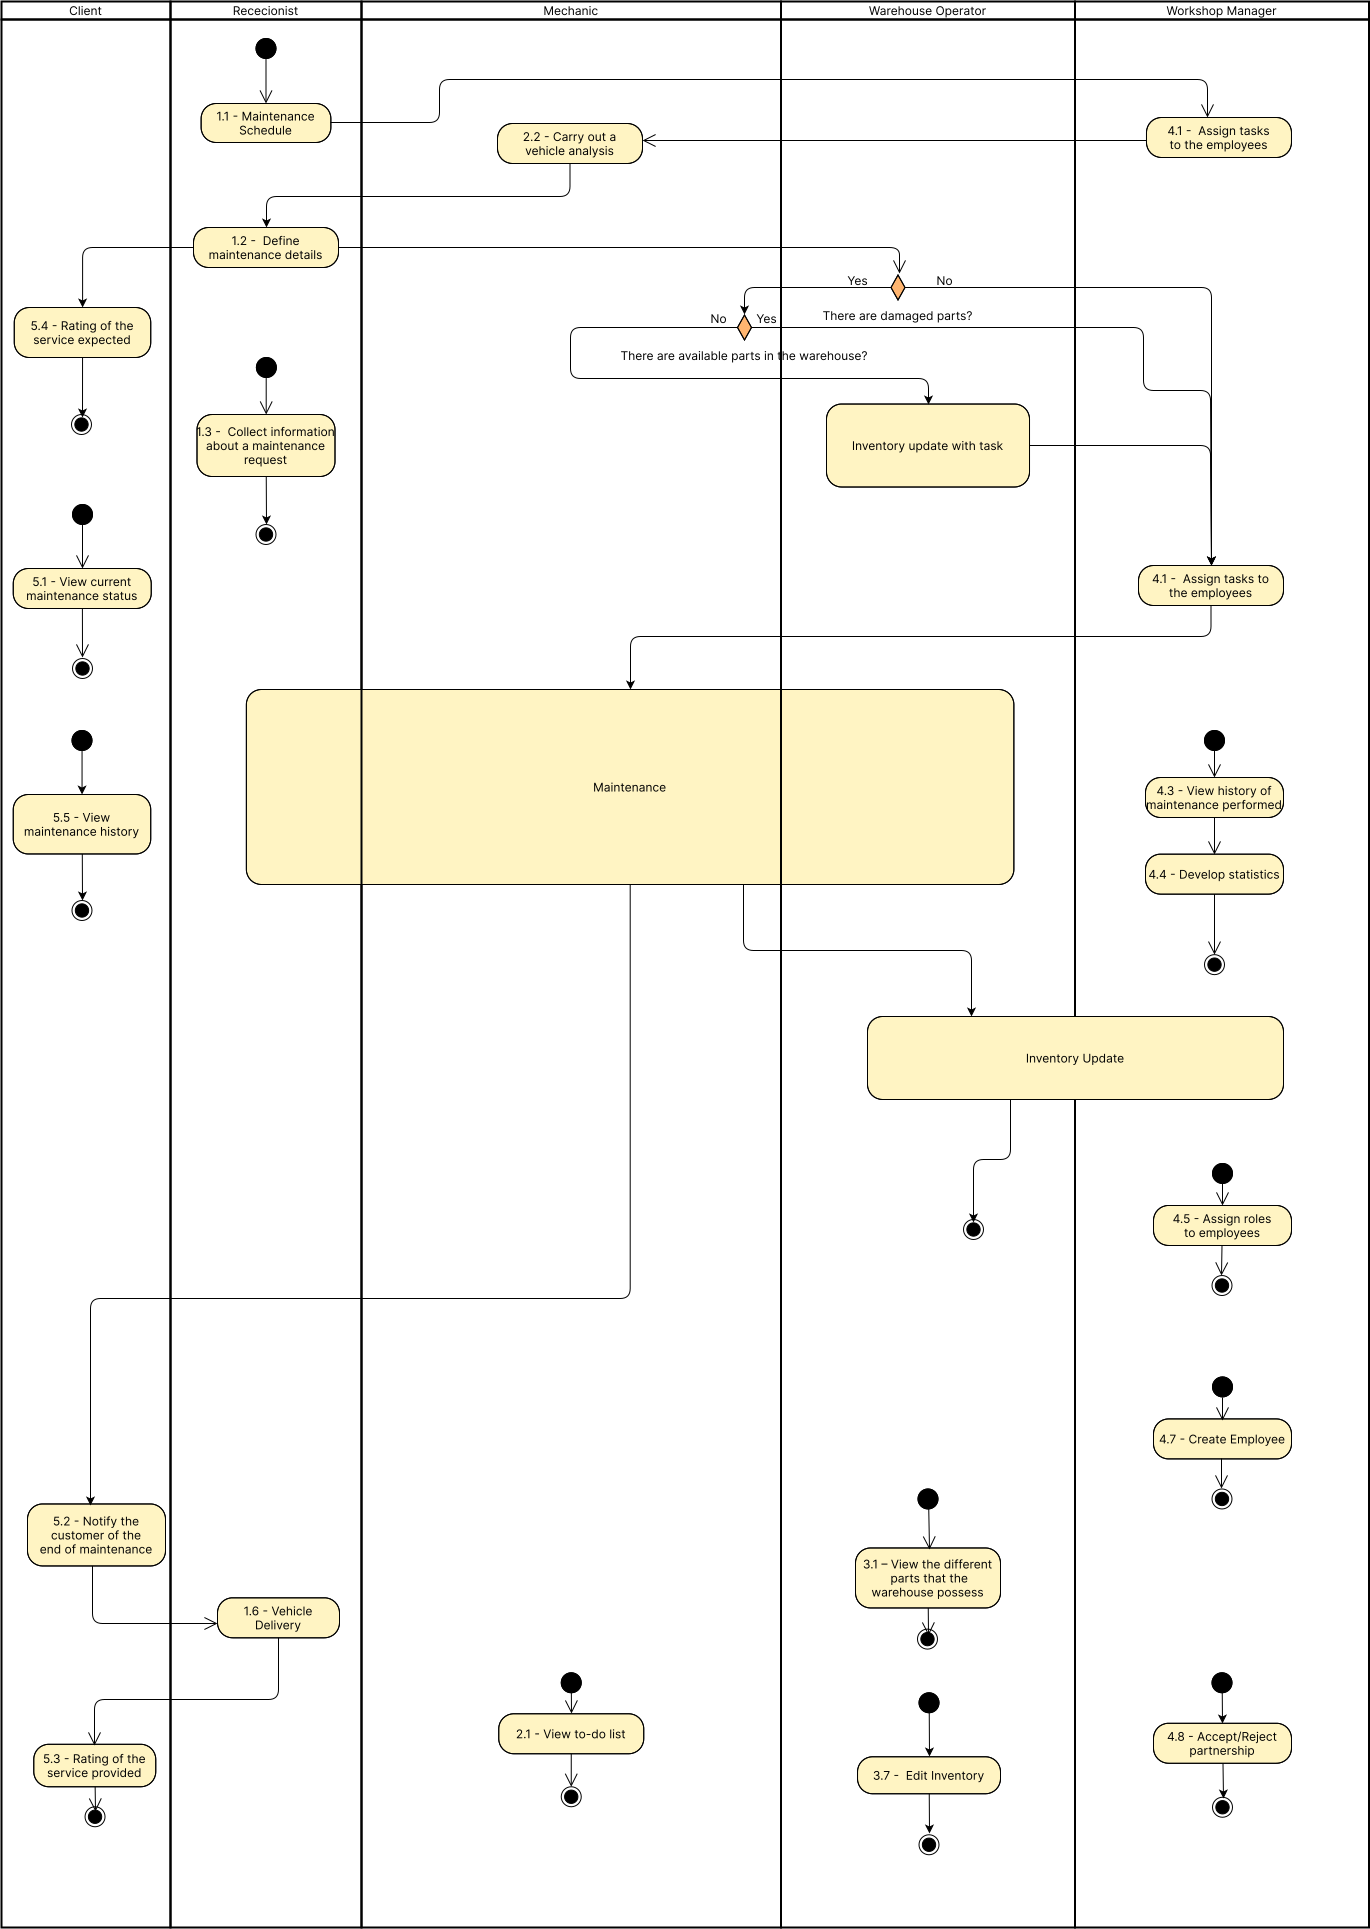
\includegraphics[width=\textwidth]{figs/UseCaseDiagram - General}
  \label{fig:figure2}
\end{figure}

The system's main flow starts when a Client arrives at the dealership for vehicle maintenance. 
The receptionist gets some input from the client and decides on an initial budget and check-out date agreed with him and inserts the information in the system (Use Case 1.1).
After that, a worker will be responsible for doing the analysis of the vehicle. 
He will add to the system all the problems he finds and the necessary parts that need to be replaced (Use Case 2.2).

When this process is complete, the rececionist contacts the client to inform these information and they both interact to achieve a mutual agreement on the maintenance procedure, conclusion date and budget (Use Case 1.2). After this, the client avaliates the service he expects to receive from the workshop (Use Case 5.4).

After this step, the manager will receive a notification of the new tasks and will assign them to each worker (Use Case 4.1).
From there on, the maintenance process can or can not require the need for a vehicle part to be replaced. 
In the negative case the vehicle goes to the responsible mechanic to do the respective task (Use Case 2.6). 
In the affirmative case, the Warehouse Operator will check if the parts the mechanic needs are available in stock. 
If they are, the mechanic receives the new parts from the operator and do the maintenance task (Use Case 2.4). 
If they aren't, the operator needs to buy new parts from the supplier. 
In this case, he initiates a new requesting purchase that can be authorized by the manager (Use Case 4.2). 
In the optimal case, the manager accepts the purchase, the operator buys the new parts (Use Case 3.3), registers them in the system (Use Case 3.4), and delivers them to the mechanic. 
In the negative scenario, the manager rejects the purchase and the process restarts with a new purchase request from the operator (Use Case 3.2).    

Until the maintenance is complete, the the budget to complete the work or the expected time may changes due to a purchase delay (Use case 3.6) or a task change (Use case 2.5). This provokes an alert to the receptionist to inform the Client. 
The result of this interaction must be "authorize the changes and continue the work" (Use Case 1.4), "not authorize the changes but continue as initially agreed"(Use Case 1.5), "not authorizing the changes and complete the remaining tasks" (Use Case 1.8) or "cancel the maintenance" (Use Case 1.7).
In the last case, all the remaining tasks are invalidated and the vehicle waits for the check-out (Use Case 5.3). 
In any other case, the maintenance process continues with the information altered.

Finally, when the vehicle maintenance is finished, the system notifies the customer that the vehicle is ready for the check out and, when the receptionist delivers the vehicle to the Customer (Use Case 1.6), the client application asks to rate the system (Use Case 5.2 and 5.3).

There are also a few secondary flows visible in the figure \ref{fig:figure2}. 
These flows are listed below:
\begin{itemize}
  \item The client enters the application to check the status of the maintenance (Use case 5.1);
  \item The mechanic enters the application to view the task he has to do (Use Case 2.1); 
  \item The rececionist enters the application to collect information to contact the client (Use Case 1.3)
  \item The Warehouse Operator enters the application to visualize the diverse parts and components in the warehouse (Use case 3.1); 
  \item The Admin enters the application to assign roles and/or permissions to the employees (Use Case 4.4); 
  \item The Admin enters the application to gather information about a maintenance performed and see statistics about that information (Use Case 4.2 and 4.3); 
\end{itemize}

 

\section{Status} 

With the flow talked in the previous section, it was needed to create multiple status of system.
- The maintenance status: the status of a maintenance
- The maintenance change status: the status when occurs a change on the maintenance like the conclusion date was changed or the budget.
- The maintenance task status: the status of a mechanic task.
- The purchase status: the status when the dealership purchase new parts
- The owner partnership status: when a bike sharing entity wants to associate with the dealership to provide maintenance of theres vehicles

\subsection{Maintenance} 


\begin{figure}[h]
  \caption{Status flow chart of a maintenance}
  \centering
  \includegraphics[width=\textwidth]{figs/Status/Maintenance/StatusDiagram}
  \label{fig:figure2}
\end{figure}


When occurr a maintenance it is divided in 6 status as seen in the figure above:
- Wait Evaluation: the inicial status when the vehicle is waiting to be analysed by the mechanic
- Wait Approval: the status where the tasks choosen by the mechanic need to be approved by the client, as well as the budget and the conclusion date
- During Maintenance: the status when the tasks of the maintenance are being done
- Maintenance Finished: after all the tasks of the maintenance are completed
- Delivered: when the vehicle is delivered to the client
- Canceled: when the client decides to cancel the maintenance and retrieve the vehicle as it is


\begin{figure}[h]
  \caption{Use case flow chart of dealership normal maintenance. With the status grouped by the use cases}
  \centering
  \includegraphics[width=\textwidth]{figs/Status/Maintenance/UseCaseStatus}
  \label{fig:figure2}
\end{figure}

In the figure above we can see how this status is divided in the flow of the use case of a maintenance in a dealership.
The flow starts with the "Wait Evaluation" status when the client contacts the rececionist to schedule a new maintenance. Then this status is hold with the assign of the evaluation task and the execution of the task by the mechanic.
When the task is done, the maintenance pass to the "Wait Approval" status where the rececionist contacts the client to confirm which tasks he decides to use in the maintenance as well as the budget and the conclusion date of the maintenance.
After the client decides which tasks he wants to keep and which he doesnt the maintenance pass to the status "During maintenance", where it keeps it until the end of the last task. Until this point the client can contact the rececionist to cancel the maintenance and pass to the status "Canceled", where the client can rate the service provided.
After the maintenance is finished, the maintenance pass to the stastus "Maintenance Finished" where the client is notified with the conclusion of the maintenance and the vehicle is delivered. After the vehicle is delivered, the maintenace pass to the status "Delivered" and the client may rate the service.

\begin{figure}[h]
  \caption{Use case flow chart of a entity with maintenance of theres vehicles. With the status grouped by the use cases}
  \centering
  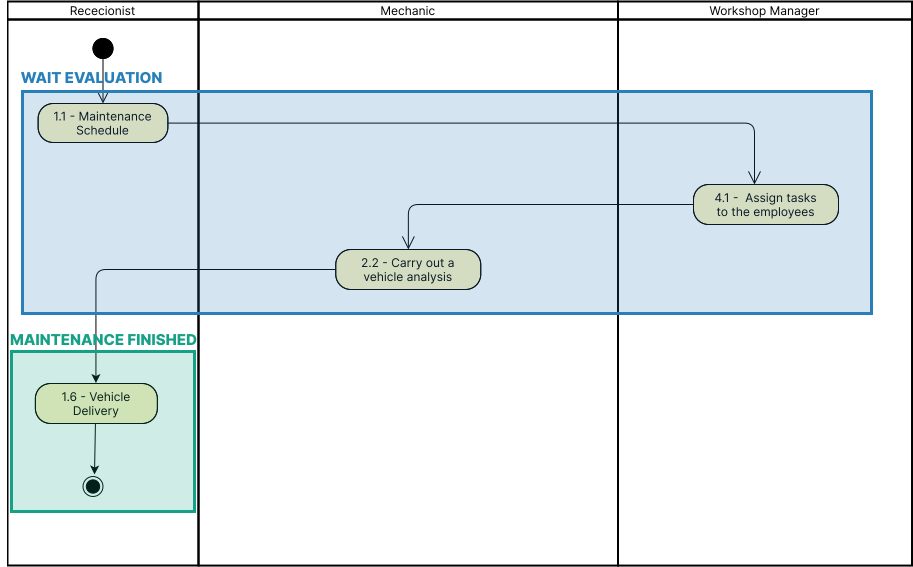
\includegraphics[width=\textwidth]{figs/Status/Maintenance/EntityDiagram}
  \label{fig:figure2}
\end{figure}

When the entity doing the maintenance also provides a bike sharing system, the maintenance may be more efficient.
In that case there is a flow of the system more simplified.
First a rececionist or another employee enconters a problem in a vehicle and schedules a maintenance with the rececionist. In this situation the maintenance is in "Wait Evaluation" status until the evaluation is carried out like the previous flow.
The diference in this flow is, during the evaluation the mechanic is not going to say which task is needed to be performed on the vehicle, he says which tasks he done during the evaluation to complete the maintenance, so the maintenance of the vehicle pass to the "Maintenance Finished" status.
Since this maintenance doesn't have a client the client is not notified so but when the vehicle leaves the workshop to the redistributors to the be used, it pass to the "Delivered" state.  


\subsection{Maintenance Change} 


\begin{figure}[h]
  \caption{Status flow chart of a maintenance Change}
  \centering
  \includegraphics[width=\textwidth]{figs/Status/MaintenanceChange/StatusDiagram}
  \label{fig:figure2}
\end{figure}


When occurr a maintenance change the client needs to be notified and this flow has the following status, as seen in the figure above:
- AskClient, The inicial status when the maintenance change needs to be confirmed by the client
- Agreed, when the client accept the changes
- Refused, when the changes are refused and the maintenance keeps the same information and the previous agreement; 
- TaskCanceled, when the client decides to cancel the task that provokes the maintenance change
- MaintenanceCanceled, when the client decides to terminated the maintenance as it is.



\begin{figure}[h]
  \caption{Use case flow chart of a maintenance change divided by the multiple status of the maintenance change}
  \centering
  \includegraphics[width=\textwidth]{figs/Status/MaintenanceChange/UseCaseStatus}
  \label{fig:figure2}
\end{figure}

In the figure above we can see how this status is divided in the flow of the use case of a maintenance change.
First a change is made in the maintenance and the rececionist is notified to contact the client, at this time the status s "Ask Client".
After contacting the client and explaining the situation the rececionist have this option depending on the will of the client:
- Agreed, when the client accept the changes
- Refused, when the changes are refused and the maintenance keeps the same information and the previous agreement; 
- TaskCanceled, when the client decides to cancel the task that provokes the maintenance change
- MaintenanceCanceled, when the client decides to terminated the maintenance as it is.

\subsection{Maintenance Task} 


\begin{figure}[h]
  \caption{Status flow chart of a task}
  \centering
  \includegraphics[width=\textwidth]{figs/Status/MaintenanceTask/StatusDiagram}
  \label{fig:figure2}
\end{figure}


In the figure above we can see how this status is divided in the flow of the use case of a task.
- WaitApproval: The inicial state when the task is created and before the approval from the client.
- WaitAssignment: The state when a task is approved by the client and has no needed parts or the parts needed are on the warehouse. 
- Invalid: When a task is rejected by the client
- Assigned: When a ready task is a assigned to a mechanic
- Concluded: When a mechanic finish concluding the task
- Changed: When the mechanic notes a problem during the task and suggest a change that requires the validation from the client
- WaitPart: When the task is aproved by the client but needs parts to be completed that are not in the inventory.



\begin{figure}[h]
  \caption{Use case flow chart of a task divided by the multiple status of the task}
  \centering
  \includegraphics[width=\textwidth]{figs/Status/MaintenanceTask/UseCaseStatus}
  \label{fig:figure2}
\end{figure}

In the figure above we can see the flow of a maintenance task during a maintenance.
The flow may start with two states, the "Wait Approval" or with the "Concluded".
On the case of a bikesharing system with maintenance of there own vehicle, the mechanic during the evaluation it completes the tasks that he registers so this tasks added to the system start at the state concluded.
At a dealership, a task from a maintenance with a client starts with the workshop manager adding a new task or during the evaluation of the maintenance.
In this time the task is in the status "Wait Approval". Then the task needs to be validated by the client. 
If it is invalidated it takes the status "Invalid" and the task flow ends here. If the task is approved, the system checks if it needs parts to be completed and if the task are available in the warehouse.
If the task need the parts and they are not available, the flow stops in the state "Wait part". After that, the system verifies if the task is assigned to a user. 
If it is not, the task holds in the state "Wait Assignment", until the workshop manager assigns a mechanic. Then, it goes to the state "Assigned", where the mechanic executes the task.
If the mechanic does not find any problens, the task is finished and goes to the state "Concluded" ending the flow. If the mechanic finds that the chosen part is not apropriate to this vehicle, he can suggest a new part to complete the task and the task goes to the state "Changed".
After this, the client needs to approve this change and the flow repeats after "Wait Approval" state.


\subsection{Purchase} 



\begin{figure}[h]
  \caption{Status flow chart of a purchase}
  \centering
  \includegraphics[width=\textwidth]{figs/Status/Purchase/StatusDiagram}
  \label{fig:figure2}
\end{figure}


When occurr a purchase the workshop manager needs to be notified and the flow has the following status, as seen in the figure above:
- WaitApproval: The inicial state when the purchase request needs to be approved by the workshop manager
- Invalid: When the workshop manager rejects a purchase request
- Assigned: When the purchase request was approved by the workshop manager and assigned to a warehouse operator
- WaitArrival: After the operator assigned to the purchase contacts the supplier to request the purchase
- Finished: When the parts arrive at the dealership and are registered into the system


\begin{figure}[h]
  \caption{Use case flow chart of a purchase divided by the multiple status of the purchase}
  \centering
  \includegraphics[width=\textwidth]{figs/Status/Purchase/UseCaseStatus}
  \label{fig:figure2}
\end{figure}

In the figure above we can see how this status is divided in the flow of the use case of a purchase.
The flow starts when the operator (or the system) makes a purchase request. This request has the state "Wait Approval" untils the workshop manager authorize (or not) the request.
If the workshop manager rejects the request, the purchase request keeps with the status "Invalid" and the flow ends here. If the purchase is authorized, purchase passes to the status "Assigned".
After the request is authorized, the warehouse operator assigned to the purchase contacts the supplier to get the parts of the request.
After that, he introduces the expected date of the Arrival of the parts and the request pass to the status "Wait Arrival".
When the parts arrive at the dealership the operator register the parts and the purchase pass to the status "Finished"


\subsection{Owner Partnership} 



\begin{figure}[h]
  \caption{Status flow chart of a partnership}
  \centering
  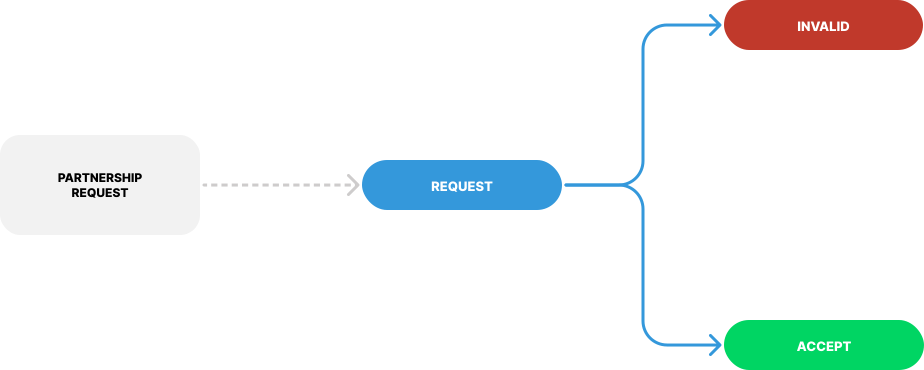
\includegraphics[width=\textwidth]{figs/Status/OwnerPartnership_StatusDiagram}
  \label{fig:figure2}
\end{figure}

when a entity wants to do a partnership with a dealership to allow him to do the maintenance of theres vehicle the flow is follow by the figure above:
- Request: the workshop manager is notified that a new entity wants to do a partnership with the dealership
- Accept, the dealership is allow to see the information about the vehicles of that entity and schedule maintenance for its vehicles
- Denied, the request was denied




